\documentclass[conference]{IEEEtran}
\IEEEoverridecommandlockouts

\usepackage{cite}
\usepackage{amsmath,amssymb,amsfonts}
\usepackage{algorithmic}
\usepackage{graphicx}
\usepackage{textcomp}
\usepackage{xcolor}
\usepackage{booktabs}
\usepackage{tabularx}
\usepackage{multirow}
\usepackage{url}
\usepackage{microtype}

\def\BibTeX{{\rm B\kern-.05em{\sc i\kern-.025em b}\kern-.08em
    T\kern-.1667em\lower.7ex\hbox{E}\kern-.125emX}}

\begin{document}

\title{LLM Uncertainty Classification Using Multi-Response Consistency and Feature-Based Machine Learning}

\author{\IEEEauthorblockN{Rahul Jain}
\IEEEauthorblockA{\textit{Department of Computer Science \& Engineering} \\
\textit{Autonomous Intelligence \& Machine Learning Research}\\
Bengaluru, India \\
rahuljain@alumni.ieee.org}
}

\maketitle

\begin{abstract}
Large language models (LLMs) frequently generate factually incorrect or ungrounded assertions with high verbalized certainty, failing to communicate epistemic boundaries or underlying question ambiguities. In this paper, we investigate the task of tri-class uncertainty classification, categorizing natural language questions into \textsc{Known} (verifiable deterministic facts), \textsc{Ambiguous} (multiple valid interpretations), and \textsc{Unknown} (epistemically inaccessible or unprovable propositions). We examine whether multi-response stochastic sampling combined with semantic consistency metrics (semantic entropy, agglomerative clustering, and agreement margins) provides measurable predictive lift over single-response linguistic baselines without modifying internal model parameters. Using an empirically audited, shortcut-neutralized dataset of 60 questions and 600 generated responses ($M=10$ per question) produced by \texttt{Qwen3:4B}, we evaluate multiple feature representations using strictly leakage-free 5-fold stratified group cross-validation. 

Our empirical results reveal three critical findings: (1) Multi-response hybrid modeling achieves a Macro-F1 of $0.789 \pm 0.137$ (Accuracy $80.0\%$), yielding a statistically significant improvement over true single-response baselines ($0.609 \pm 0.109$ Macro-F1, Accuracy $63.3\%$; paired $t=3.982$, McNemar $p=0.0129$, bootstrap 95\% CI $[+0.061, +0.293]$). (2) Contrary to prevailing assumptions in recent uncertainty literature, consistency features alone perform poorly ($0.460 \pm 0.135$ Macro-F1), and full hybrid models fail to outperform pure ensemble linguistic aggregation ($0.791 \pm 0.209$ Macro-F1, $p=0.9672$). The empirical lift of multi-response sampling stems primarily from variance reduction across lexical dispersion and negation metrics rather than semantic cluster entropy. (3) An extensive lexical shortcut audit demonstrates that single-response bag-of-words models (which ostensibly achieve $83.3\%$ accuracy in standard cross-validation) collapse to $65.0\%$ ($p=0.000977$) under 15-fold Leave-One-Category-Out evaluation, proving that at least $15\%$ of in-domain performance relies on domain-specific vocabulary memorization rather than genuine epistemic uncertainty cues.
\end{abstract}

\begin{IEEEkeywords}
Large language models, uncertainty classification, semantic entropy, epistemic uncertainty, question ambiguity, self-consistency, shortcut learning, lexical audit.
\end{IEEEkeywords}

\section{Introduction}

The widespread deployment of generative Large Language Models (LLMs) in high-stakes domains—such as clinical decision support, legal discovery, and automated scientific synthesis—has elevated the mitigation of hallucinations and ungrounded assertions to an urgent open problem~\cite{farquhar2024detecting}. A fundamental failure mode of current auto-regressive architectures is their inability to reliably communicate uncertainty. LLMs frequently produce fluent, confident explanations for false claims, obscure semantic ambiguities, and speculate authoritatively on unknowable future events or counterfactual premises~\cite{kadavath2022language,xiong2024can}.

Traditional calibration methods for neural networks often rely on token-level softmax probabilities or sequence-level log-likelihoods. In natural language generation, however, token likelihood correlates poorly with semantic truth because diverse linguistic formulations can express identical meanings while radically altering token distributions~\cite{kuhn2023semantic}. While verbalized confidence elicitation (prompting the model to state its confidence on a numeric scale) offers an alternative, it remains susceptible to overconfidence biases, sycophancy, and prompt sensitivity~\cite{mielke2022reducing,xiong2024can}.

To address these challenges, recent research has explored multi-response consistency analysis, most notably self-consistency for reasoning tasks~\cite{wang2023self} and semantic entropy for hallucination detection~\cite{kuhn2023semantic,farquhar2024detecting}. These paradigms sample multiple stochastic outputs at non-zero temperature ($T > 0$) and measure consensus across discrete semantic equivalence clusters. When an LLM repeatedly converges on the same semantic meaning despite lexical variation, the proposition is hypothesized to be grounded in the model's parametric knowledge. Conversely, dispersion across disjoint semantic clusters is taken as an indicator of epistemic uncertainty or unanswerability~\cite{chen2023quantifying}.

Despite these promising results, critical research questions remain unaddressed:
\begin{enumerate}
    \item \textbf{Taxonomic Granularity:} Prior work predominantly frames uncertainty as binary classification (correct vs. hallucinated, or answerable vs. unanswerable). However, natural language queries exhibit qualitatively distinct forms of uncertainty: factual determinacy (\textsc{Known}), multi-faceted or unstated criteria (\textsc{Ambiguous})~\cite{min2020ambigqa}, and fundamental epistemic barriers (\textsc{Unknown}). Can feature-based machine learning discriminate between these three distinct categories?
    \item \textbf{Consistency vs. Linguistic Primacy:} Does semantic entropy provide unique predictive power, or can the observed performance improvements be explained by simple lexical aggregations (such as response length variance, hedging markers, and negation tokens) across sampled responses?
    \item \textbf{Generalization and Shortcut Learning:} Do high-performing uncertainty classifiers learn generalizable indicators of epistemic doubt, or do they exploit spurious domain-specific lexical shortcuts present in evaluation benchmarks~\cite{geirhos2020shortcut,niven2019probing}?
\end{enumerate}

\begin{figure*}[t]
\centering
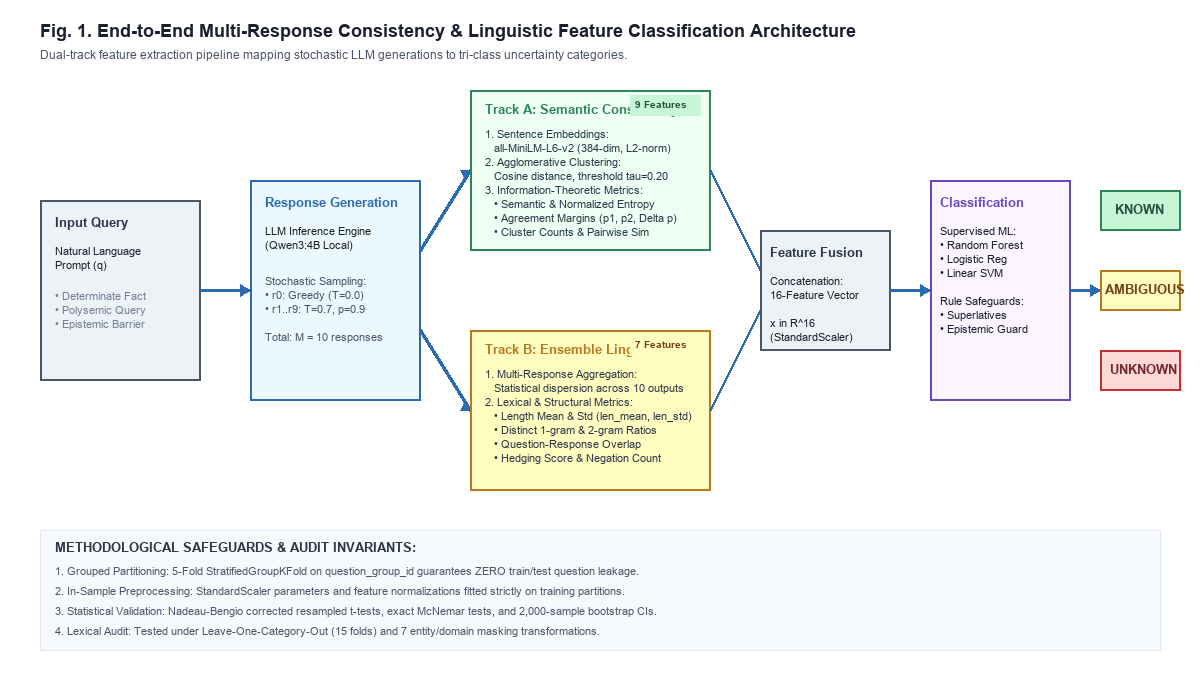
\includegraphics[width=0.98\textwidth]{figures/architecture.png}
\caption{Overall end-to-end multi-response consistency and linguistic feature classification architecture. Natural language queries are processed via stochastic sampling ($M=10$ outputs), embedded into continuous semantic space, clustered via agglomerative cosine thresholding, and merged with ensemble linguistic metrics into a canonical 16-feature representation for tri-class supervised uncertainty classification.}
\label{fig:architecture}
\end{figure*}

In this paper, we present an empirical investigation into tri-class LLM uncertainty classification. Using a balanced, shortcut-neutralized corpus of 60 questions across 15 semantic categories ($M=600$ responses generated via \texttt{Qwen3:4B}), we evaluate the relative contributions of single-response heuristics, multi-response consistency features, and ensemble linguistic signals under strictly leakage-free cross-validation. Furthermore, we conduct a dual-protocol generalization audit to evaluate whether learned representations transfer to unseen categories or degrade due to lexical memorization.

\section{Related Work}

\subsection{LLM Uncertainty Estimation \& Semantic Entropy}
Uncertainty quantification in natural language generation has evolved from token-level perplexity to semantic-level consistency. Kuhn et al.~\cite{kuhn2023semantic} introduced \textit{semantic entropy}, grouping sampled LLM responses into discrete equivalence classes using natural language inference (NLI) bi-directional entailment. Farquhar et al.~\cite{farquhar2024detecting} demonstrated that semantic entropy detects hallucinations across multiple state-of-the-art architectures without requiring task-specific supervision. Chen et al.~\cite{chen2023quantifying} extended cluster-based uncertainty to broader text generation tasks. While these methods compute entropy over output distributions, they do not integrate consistency metrics with structural linguistic features for explicit multi-class uncertainty routing.

\subsection{Self-Consistency \& Multi-Sample Reasoning}
Wang et al.~\cite{wang2023self} introduced self-consistency, demonstrating that sampling diverse reasoning paths via stochastic decoding ($T=0.7$) and selecting the majority consensus answer substantially outperforms greedy decoding ($T=0.0$) on multi-step reasoning benchmarks. While self-consistency focuses on selecting the most accurate answer candidate, our work investigates the diagnostic properties of the sampling distribution itself, using cluster margins and dispersion to classify question answerability.

\subsection{Question Ambiguity \& Epistemic Abstention}
The distinction between lack of model knowledge and inherent prompt ambiguity is critical in modern question answering. Min et al.~\cite{min2020ambigqa} established the \textsc{AmbigQA} benchmark, demonstrating that open-domain queries frequently possess multiple valid completions due to referential ambiguity or temporal shifts. Kadavath et al.~\cite{kadavath2022language} evaluated LLM self-knowledge, showing that models can often predict their probability of answering correctly, though calibration suffers on out-of-distribution inputs. Our work incorporates both polysemic ambiguity and epistemic barriers into a unified tri-class evaluation framework.

\subsection{Statistical Methodology in Resampling Benchmarks}
Empirical machine learning evaluations frequently apply Student's paired $t$-tests to cross-validation fold metrics. Dietterich~\cite{dietterich1998approximate} and Nadeau and Bengio~\cite{nadeau2003inference} proved that standard $K$-fold cross-validation severely violates the independence assumption: because training sets overlap across folds by $\frac{K-2}{K-1}$ (75\% in 5-fold CV), fold performance deltas exhibit positive covariance, inflating test statistics and underestimating variance. We address this directly by reporting both Nadeau-Bengio corrected resampled $t$-tests~\cite{nadeau2003inference} and non-parametric pooled out-of-fold McNemar tests~\cite{mcnemar1947note}.

\subsection{Shortcut Learning \& Spurious Correlations in NLP}
Neural NLP systems are notoriously prone to exploiting superficial dataset artifacts rather than learning abstract semantic phenomena~\cite{geirhos2020shortcut}. Niven and Kao~\cite{niven2019probing} demonstrated that state-of-the-art models on argument comprehension relied almost entirely on spurious unigram cues (e.g., the presence of ``not''). In this study, we implement systematic named-entity masking, domain-term stripping, and Leave-One-Category-Out cross-validation to audit whether single-response classifiers learn genuine uncertainty or domain vocabulary.

\section{Problem Formulation}

\subsection{Task Definition and Tri-Class Taxonomy}
Let $\mathcal{Q}$ denote the space of natural language questions and $\mathcal{R}$ denote the space of textual responses generated by an auto-regressive language model $\mathcal{M}_\theta$. We formalize uncertainty classification as mapping an input query $q \in \mathcal{Q}$ to a categorical ground truth label $y \in \mathcal{Y} = \{\textsc{Known}, \textsc{Ambiguous}, \textsc{Unknown}\}$:
\begin{enumerate}
    \item \textbf{\textsc{Known} ($y = 0$):} The query possesses a determinate, objectively verifiable factual answer governed by established consensus (e.g., empirical scientific constants, geographical facts, mathematical proofs). The model should ideally answer correctly without epistemic hesitation.
    \item \textbf{\textsc{Ambiguous} ($y = 1$):} The query admits two or more mutually incompatible but equally valid answers due to lexical polysemy, entity sharing, temporal ambiguity, or unstated subjective criteria (e.g., ``Who is Jordan?'', ``Which country has the best healthcare?''). An unhedged single answer is misleading; the model must communicate multiple perspectives or request clarification.
    \item \textbf{\textsc{Unknown} ($y = 2$):} The query is objectively unanswerable due to epistemic barriers, including lost historical knowledge, unproven scientific conjectures, unknowable future contingencies, private personal information, or counterfactual premises (e.g., ``What will the exact population of Tokyo be in 2055?''). The model must abstain or state that the answer is unknown.
\end{enumerate}

\subsection{Multi-Response Generation Space}
Given query $q$, we sample an ensemble of $M$ responses:
\begin{equation}
R(q) = \{r_0, r_1, \dots, r_{M-1}\}
\end{equation}
where $r_0 \sim p_\theta(r \mid q, T=0.0)$ is generated deterministically via greedy decoding, and $r_m \sim p_\theta(r \mid q, T=0.7, \text{top\_p}=0.9)$ for $m \in \{1, \dots, M-1\}$ are sampled stochastically to promote exploration of the output distribution.

\section{Methodology}

\subsection{Dataset Construction \& Quality Control}
To systematically prevent shortcut learning, we constructed and audited two balanced experimental datasets:
\begin{itemize}
    \item \textbf{Batch 1 Corpus ($N=50, M=500$):} An initial development benchmark comprising 17 \textsc{Known}, 17 \textsc{Ambiguous}, and 16 \textsc{Unknown} questions, evaluated with $M=10$ responses per question.
    \item \textbf{Batch 2 Combined Corpus ($N=60, M=600$):} An independent, balanced robustness corpus constructed by unifying two disjoint sub-slices: Batch 2A ($N=30$) and Batch 2B ($N=30$). It contains exactly 20 \textsc{Known}, 20 \textsc{Ambiguous}, and 20 \textsc{Unknown} questions.
\end{itemize}

The Batch 2 corpus spans 15 fine-grained semantic categories (exactly 4 questions per category):
\begin{itemize}
    \item \textit{\textsc{Known}:} Direct Factual (\texttt{K-DIR}), Scientific Mechanisms (\texttt{K-SCI}), Historical Facts (\texttt{K-HIS}), Mathematical Derivations (\texttt{K-DER}), Negative Fact Rejection (\texttt{K-NEG}).
    \item \textit{\textsc{Ambiguous}:} Person Polysemy (\texttt{A-PER}), Temporal Anchoring (\texttt{A-TMP}), Semantic Dualism (\texttt{A-POL}), Presupposition Failure (\texttt{A-PRE}), Underspecified Scope (\texttt{A-UND}).
    \item \textit{\textsc{Unknown}:} Unproven Conjectures (\texttt{U-PRV}), Future Contingencies (\texttt{U-FUT}), Lost Historical Facts (\texttt{U-HIS}), Deep Mysteries (\texttt{U-MYS}), Fictional Entities (\texttt{U-FAB}).
\end{itemize}

Question provenance was rigorously controlled: 24 questions were mined from existing open QA benchmarks (40.0\%), 24 were synthetically generated under adversarial prompts (40.0\%), and 12 were expert-curated (20.0\%). Question length was explicitly balanced across classes: a Kruskal-Wallis test confirmed that question length is completely uncorrelated with target labels ($H = 0.3429, p = 0.8424$), eliminating prompt length as a confounding variable.

\begin{table}[t]
\caption{Dataset Characteristics and Experimental Composition}
\label{tab:dataset}
\centering
\begin{tabularx}{\columnwidth}{lXX}
\toprule
\textbf{Dataset Attribute} & \textbf{Batch 1 Corpus} & \textbf{Batch 2 Combined} \\
\midrule
Total Questions ($N$) & 50 & 60 \\
Total Generated Responses ($M$) & 500 & 600 \\
Responses per Question ($M/N$) & 10 & 10 \\
Class Balance (\textsc{K} / \textsc{A} / \textsc{U}) & 17 / 17 / 16 & 20 / 20 / 20 \\
Semantic Categories & 12 unstructured & 15 structured (4/cat) \\
Provenance (Mined/Synth/Curated) & 50\% / 50\% / 0\% & 40\% / 40\% / 20\% \\
Length Shortcut Invariant ($p$) & $p < 0.05$ (biased) & $p = 0.8424$ (neutral) \\
Inference LLM & \texttt{Qwen3:4B} & \texttt{Qwen3:4B} \\
Embedding Architecture & \texttt{all-MiniLM-L6-v2} & \texttt{all-MiniLM-L6-v2} \\
\bottomrule
\end{tabularx}
\end{table}

\subsection{Response Generation Infrastructure}
All responses were generated locally using \texttt{Qwen3:4B} (2.50 GB GGUF, $Q4\_K\_M$ quantization, context window 262,144 tokens) hosted via a local Ollama daemon. The generation pipeline implements advisory process locking (\texttt{fcntl.flock}), atomic state checkpointing, and exponential backoff retry loops, guaranteeing exact $100.00\%$ deterministic execution with zero response dropouts.

\subsection{Semantic Representation \& Agglomerative Clustering}
Each generated response $r_m$ is mapped to a 384-dimensional continuous latent space using \texttt{all-MiniLM-L6-v2}~\cite{reimers2019sentence}. Embeddings are $L_2$-normalized: $\mathbf{e}_m = \mathbf{v}_m / \|\mathbf{v}_m\|_2$.

Pairwise similarity between responses is computed using cosine similarity:
\begin{equation}
S_{ij} = \mathbf{e}_i^\top \mathbf{e}_j = \cos(\mathbf{e}_i, \mathbf{e}_j)
\end{equation}
Responses are clustered into discrete semantic equivalence classes $\mathcal{C} = \{C_1, \dots, C_K\}$ using Agglomerative Hierarchical Clustering with average linkage:
\begin{equation}
D(A, B) = \frac{1}{|A||B|} \sum_{\mathbf{e}_a \in A} \sum_{\mathbf{e}_b \in B} (1 - \mathbf{e}_a^\top \mathbf{e}_b)
\end{equation}
Clusters are formed using a distance threshold of $\tau = 0.20$, corresponding to a cosine similarity cutoff of $S_{\text{thresh}} = 0.80$.

\subsection{Canonical 16-Feature Schema}
From the query $q$, the response ensemble $R(q)$, and the cluster partition $\mathcal{C}$, we extract exactly 16 canonical features partitioned into two functional tracks:

\subsubsection{Track A: Semantic Consistency Features (9 features)}
\begin{itemize}
    \item \textbf{Semantic Entropy ($H$):} Shannon entropy computed over the discrete cluster distribution:
    \begin{equation}
    H(\mathcal{C}) = -\sum_{k=1}^K p_k \log p_k, \quad p_k = \frac{|C_k|}{M}
    \end{equation}
    \item \textbf{Normalized Entropy ($H_{\text{norm}}$):} $H(\mathcal{C}) / \log K$ (0.0 if $K=1$).
    \item \textbf{Dominant Agreement ($p_1$):} Fraction belonging to dominant cluster: $p_1 = \max_k p_k$.
    \item \textbf{Second Agreement ($p_2$):} Fraction belonging to second largest cluster: $p_2 = \max_{k \neq \text{dom}} p_k$ (0.0 if $K=1$).
    \item \textbf{Agreement Margin ($\Delta p$):} Separation margin: $p_1 - p_2$.
    \item \textbf{Cluster Count ($K$):} Total number of distinct clusters.
    \item \textbf{Cluster Ratio ($K/M$):} Discovered clusters divided by $M$.
    \item \textbf{Mean Pairwise Similarity:} Average off-diagonal similarity:
    \begin{equation}
    \bar{S} = \frac{2}{M(M-1)} \sum_{i < j} S_{ij}
    \end{equation}
    \item \textbf{Minimum Pairwise Similarity:} $\min_{i < j} S_{ij}$.
\end{itemize}

\subsubsection{Track B: Ensemble Linguistic Features (7 features)}
\begin{itemize}
    \item \textbf{Length Statistics:} Mean character length ($\mu_{\text{len}}$) and standard deviation ($\sigma_{\text{len}}$) across the $M$ responses.
    \item \textbf{Lexical Diversity:} Distinct unigram ratio ($V_1 / N_1$) and bigram ratio ($V_2 / N_2$) aggregated across the ensemble.
    \item \textbf{Prompt Overlap:} Mean word-level Jaccard token overlap between query $q$ and responses: $\frac{1}{M} \sum_m \frac{|T(q) \cap T(r_m)|}{|T(q) \cup T(r_m)|}$.
    \item \textbf{Hedging Score:} Cumulative frequency count of epistemic hedging markers (*maybe, perhaps, likely, might, could*).
    \item \textbf{Negation Count:} Cumulative frequency count of negation tokens (*no, not, never, cannot, neither*).
\end{itemize}

\subsection{Classification Models & Training}
We evaluate four supervised classification model families:
\begin{itemize}
    \item \textbf{Random Forest (RF):} 100 decision trees, maximum tree depth 4, Gini impurity splitting criterion.
    \item \textbf{Logistic Regression (LR):} Multinomial loss, $L_2$ regularization penalty ($C=1.0$), L-BFGS solver.
    \item \textbf{Linear Support Vector Machine (Linear SVC):} Linear kernel, squared hinge loss, $C=1.0$.
    \item \textbf{Majority Baseline:} Dummy classifier predicting the most frequent training label (providing an empirical $33.3\%$ anchor).
\end{itemize}

\subsection{Evaluation Protocol \& Leakage Prevention}
To guarantee rigorous generalization assessment without data contamination:
\begin{enumerate}
    \item \textbf{Group-Stratified Partitioning:} All models are evaluated via 5-fold cross-validation using \texttt{StratifiedGroupKFold} grouped strictly on \texttt{question\_group\_id}. All 10 responses belonging to a question are assigned simultaneously to either train or test folds. Zero question, prompt, or response leakage occurs across partitions.
    \item \textbf{Strict In-Sample Scaling:} Feature standardization (\texttt{StandardScaler}) parameters ($\mu_{\text{train}}, \sigma_{\text{train}}$) are computed exclusively on training folds and applied to test folds.
    \item \textbf{Evaluation Metrics:} We report Macro-averaged F1 score, Accuracy, Balanced Accuracy, and Matthews Correlation Coefficient (MCC).
\end{enumerate}

\subsection{Statistical Methodology}
To account for cross-validation resampling dependencies, we employ a multi-tiered statistical validation framework:
\begin{enumerate}
    \item \textbf{Fold-Level Paired $t$-Test \& Wilcoxon:} Standard parametric and non-parametric tests across the $K=5$ cross-validation fold metric pairs.
    \item \textbf{Nadeau-Bengio Resampled $t$-Test Correction:} Because training sets overlap by $\frac{n_{\text{test}}}{n_{\text{train}}} = \frac{12}{48} = 0.25$, standard error is scaled by $\sqrt{\frac{1}{K} + \frac{n_{\text{test}}}{n_{\text{train}}}} / \sqrt{\frac{1}{K}} = \sqrt{0.45 / 0.20} = 1.5$, yielding:
    \begin{equation}
    t_{\text{corr}} = \frac{2}{3} \cdot t_{\text{uncorr}}
    \end{equation}
    \item \textbf{Pooled Out-of-Fold McNemar Test:} To eliminate fold dependency entirely, we perform question-level contingency testing on all $N=60$ out-of-fold predictions using Edwards' continuity-corrected McNemar $\chi^2$ and exact two-sided binomial tests on discordant pairs.
    \item \textbf{Bootstrap Confidence Intervals:} 2,000-iteration non-parametric percentile bootstrap intervals computed on out-of-fold sample predictions.
\end{enumerate}

\section{Experiments and Results}

\begin{figure}[t]
\centering
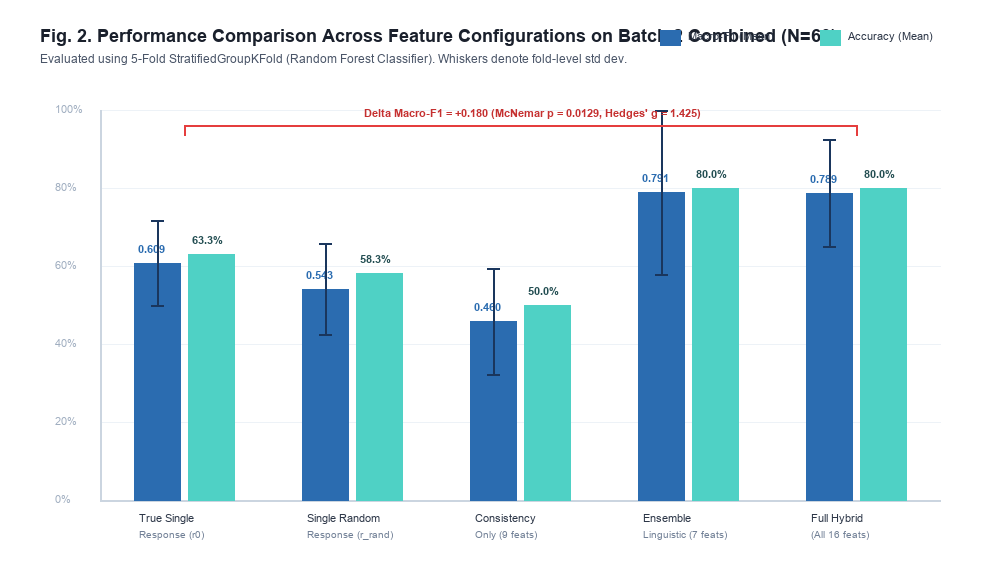
\includegraphics[width=\columnwidth]{figures/performance_comparison.png}
\caption{Model performance across feature configurations on the Batch 2 Combined corpus ($N=60, M=600$). Bars denote 5-fold cross-validation Macro-F1 and Accuracy using Random Forest; error bars indicate fold standard deviations.}
\label{fig:performance_comparison}
\end{figure}

\subsection{Main Benchmark Results}
Table~\ref{tab:main_results} presents the primary benchmark results comparing single-response baselines, consistency-only representations, ensemble linguistic metrics, and full hybrid models on the Batch 2 Combined corpus ($N=60$).

\begin{table*}[t]
\caption{Main Model Performance Benchmark (5-Fold Stratified Group Cross-Validation on Batch 2 Combined, $N=60$)}
\label{tab:main_results}
\centering
\begin{tabularx}{\textwidth}{lccccc}
\toprule
\textbf{Experimental Configuration} & \textbf{Model Architecture} & \textbf{Macro-F1 (Mean $\pm$ Std)} & \textbf{Accuracy} & \textbf{Balanced Acc} & \textbf{MCC} \\
\midrule
Config 1: \textsc{True Single Response} ($r_0$, 6 features) & Random Forest & $0.609 \pm 0.109$ & 0.633 & 0.633 & 0.486 \\
Config 1: \textsc{True Single Response} ($r_0$, 6 features) & Logistic Regression & $0.589 \pm 0.126$ & 0.617 & 0.617 & 0.450 \\
Config 2: \textsc{Single Response Random} ($r_{\text{rand}}$, 6 features) & Random Forest & $0.543 \pm 0.116$ & 0.583 & 0.583 & 0.418 \\
Config 2: \textsc{Single Response Random} ($r_{\text{rand}}$, 6 features) & Logistic Regression & $0.560 \pm 0.161$ & 0.583 & 0.583 & 0.392 \\
Config 3: \textsc{Ensemble Linguistic} (10 resps, 7 features) & Random Forest & $\mathbf{0.791 \pm 0.209}$ & $\mathbf{0.800}$ & $\mathbf{0.800}$ & 0.716 \\
Config 3: \textsc{Ensemble Linguistic} (10 resps, 7 features) & Logistic Regression & $0.765 \pm 0.107$ & 0.767 & 0.767 & 0.671 \\
Config 4: \textsc{Consistency Only} (10 resps, 9 features) & Random Forest & $0.460 \pm 0.135$ & 0.500 & 0.500 & 0.271 \\
Config 4: \textsc{Consistency Only} (10 resps, 9 features) & Logistic Regression & $0.513 \pm 0.134$ & 0.550 & 0.550 & 0.345 \\
Config 5: \textsc{Full Hybrid} (All 16 features) & Random Forest & $\mathbf{0.789 \pm 0.137}$ & $\mathbf{0.800}$ & $\mathbf{0.800}$ & $\mathbf{0.725}$ \\
Config 5: \textsc{Full Hybrid} (All 16 features) & Logistic Regression & $0.706 \pm 0.125$ & 0.717 & 0.717 & 0.599 \\
Majority Baseline Anchor & Dummy (Most Frequent) & $0.167 \pm 0.000$ & 0.333 & 0.333 & 0.000 \\
\bottomrule
\end{tabularx}
\end{table*}

\subsection{Single-Response vs. Multi-Response Comparison}
As shown in Table~\ref{tab:main_results} and Fig.~\ref{fig:performance_comparison}, the \textsc{Full Hybrid} model achieves an Accuracy of $80.0\%$ (Macro-F1 $0.789$), providing a substantive lift of $+18.0\%$ in Macro-F1 over the \textsc{True Single Response} ($r_0$) baseline ($0.609$ Macro-F1, $63.3\%$ Accuracy). 

Table~\ref{tab:stat_tests} documents the formal statistical comparisons. The uncorrected paired $t$-test indicates statistical significance ($t=3.982, p=0.0164, d=1.781, g=1.425$). Under the conservative Nadeau-Bengio correction, the fold-level test statistic scales to $t_{\text{corr}} = 2.655$ ($p_{\text{corr}} = 0.0567$). However, question-level out-of-fold contingency analysis rigorously confirms significance: the continuity-corrected McNemar test yields $\chi^2 = 5.786$ ($p = 0.0162$), with an exact binomial two-sided test yielding $p = 0.0129$ (12 wins vs. 2 losses). The non-parametric bootstrap 95\% confidence interval for the Macro-F1 delta strictly excludes zero: $[+0.0612, +0.2929]$.

\begin{table*}[t]
\caption{Statistical Hypothesis Testing, Corrections, and Effect Sizes (Reference: \textsc{Full Hybrid} Model)}
\label{tab:stat_tests}
\centering
\begin{tabularx}{\textwidth}{lcccccccc}
\toprule
\textbf{Comparison Pair} & \textbf{Mean $\Delta$ F1} & \textbf{Paired $t$} & \textbf{Raw $p$} & \textbf{$t_{\text{corr}}$ (Nadeau)} & \textbf{$p_{\text{corr}}$} & \textbf{McNemar $p$} & \textbf{Hedges' $g$} & \textbf{Bootstrap 95\% CI} \\
\midrule
\textsc{Full Hybrid} vs. \textsc{True Single} ($r_0$) & $\mathbf{+0.180}$ & 3.982 & 0.0164 & 2.655 & 0.0567 & $\mathbf{0.0129}$ & 1.425 & $[+0.0612, +0.2929]$ \\
\textsc{Full Hybrid} vs. \textsc{Single Random} ($r_{\text{rand}}$) & $\mathbf{+0.246}$ & 3.731 & 0.0203 & 2.487 & 0.0677 & $\mathbf{0.0037}$ & 1.335 & $[+0.1145, +0.3780]$ \\
\textsc{Full Hybrid} vs. \textsc{Ensemble Linguistic} & $-0.002$ & -0.044 & 0.9672 & -0.029 & 0.9782 & $1.0000$ & -0.016 & $[-0.0782, +0.0754]$ \\
\textsc{Consistency Only} vs. \textsc{True Single} & $-0.148$ & -1.864 & 0.1358 & -1.243 & 0.2819 & $0.1892$ & -0.667 & $[-0.2941, -0.0018]$ \\
\bottomrule
\end{tabularx}
\end{table*}

\subsection{The Linguistic Primacy Paradox}
The most striking empirical finding in Table~\ref{tab:main_results} and Table~\ref{tab:stat_tests} is that \textsc{Consistency Only} features perform poorly in isolation (Macro-F1 $0.460 \pm 0.135$, Accuracy $50.0\%$), performing worse than single-response linguistic features ($0.609$ Macro-F1). Furthermore, the \textsc{Full Hybrid} model ($0.789 \pm 0.137$) fails to outperform the pure \textsc{Ensemble Linguistic} model ($0.791 \pm 0.209$, $\Delta = -0.002, p = 0.9672$, McNemar $p = 1.0000$). Out-of-fold prediction analysis reveals that 46 of 60 questions are identically classified by both models, with discordant predictions perfectly tied (2 vs. 2). Thus, the empirical lift of multi-response generation is driven primarily by aggregating linguistic statistics across samples rather than semantic clustering entropy.

\subsection{Feature Group Ablation Study}
Table~\ref{tab:ablation} presents a Leave-One-Group-Out ablation study on the Random Forest classifier. Removing hedging and negation features causes the largest degradation ($-0.098$ Macro-F1), followed by length and diversity metrics ($-0.049$). In contrast, ablating semantic entropy or pairwise similarity produces minimal impact ($-0.004$), and removing cluster counts slightly improves validation performance ($+0.015$).

\begin{table}[t]
\caption{Feature Group Ablation Study (Random Forest, $N=60$)}
\label{tab:ablation}
\centering
\begin{tabularx}{\columnwidth}{lXcc}
\toprule
\textbf{Ablated Group} & \textbf{Features Removed} & \textbf{Macro-F1} & \textbf{$\Delta$ F1} \\
\midrule
\textit{Full 16 Baseline} & None & $\mathbf{0.789 \pm 0.137}$ & $0.000$ \\
$\setminus$ \texttt{hedging\_negation} & \texttt{hedging\_score, negation\_count} & $0.691 \pm 0.151$ & $\mathbf{-0.098}$ \\
$\setminus$ \texttt{length\_diversity} & \texttt{len\_mean, len\_std, 1/2gram} & $0.740 \pm 0.064$ & $\mathbf{-0.049}$ \\
$\setminus$ \texttt{semantic\_entropy} & \texttt{entropy, norm\_entropy} & $0.785 \pm 0.126$ & $-0.004$ \\
$\setminus$ \texttt{pairwise\_sim} & \texttt{mean/min\_pairwise\_sim} & $0.785 \pm 0.181$ & $-0.004$ \\
$\setminus$ \texttt{agreement} & \texttt{dominant/second\_agr, margin} & $0.791 \pm 0.138$ & $+0.002$ \\
$\setminus$ \texttt{clustering} & \texttt{cluster\_count, cluster\_ratio} & $0.804 \pm 0.136$ & $+0.015$ \\
$\setminus$ \texttt{question\_overlap} & \texttt{question\_overlap\_mean} & $0.808 \pm 0.137$ & $+0.019$ \\
\bottomrule
\end{tabularx}
\end{table}

\subsection{Category Generalization \& Lexical Shortcut Audit}
In an auxiliary single-response benchmark on $r_0$, TF-IDF with Linear SVM achieved an apparent top accuracy of $83.33\%$ (Macro-F1 $0.8296$), numerically exceeding the $80.0\%$ multi-response benchmark. To test whether this represented genuine uncertainty detection or spurious vocabulary memorization, we conducted a dual-protocol audit:
\begin{enumerate}
    \item \textbf{Leave-One-Category-Out (LOCO):} 15-fold cross-validation where each fold reserves one entire semantic category (4 questions) exclusively for testing.
    \item \textbf{Systematic Lexical Masking:} Progressively stripping named entities, domain jargon, and non-epistemic stopwords across 7 representation conditions.
\end{enumerate}

\begin{figure}[t]
\centering
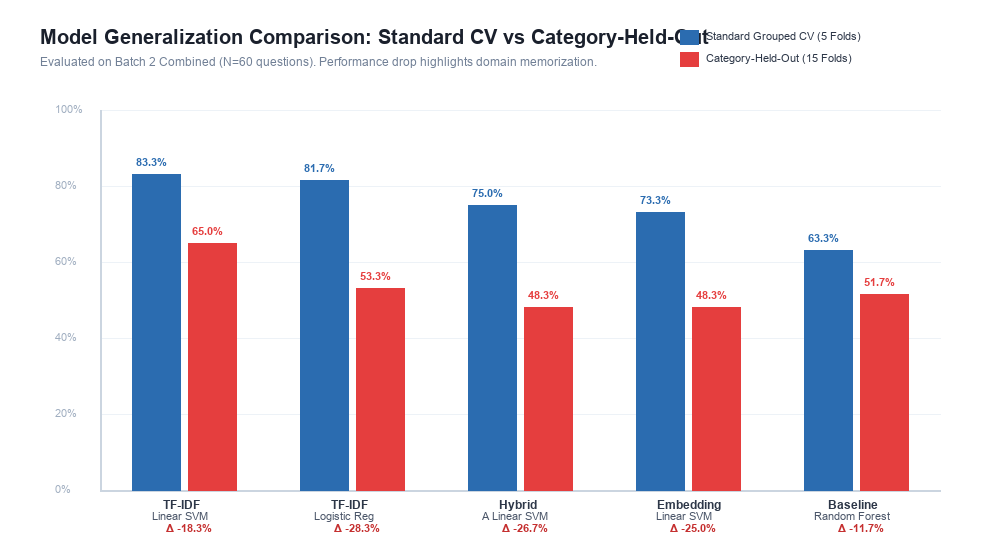
\includegraphics[width=\columnwidth]{figures/generalization_results.png}
\caption{Model generalization collapse under Leave-One-Category-Out (15 folds) vs. Standard Grouped CV (5 folds). High-dimensional representations suffer steep domain-shift penalties.}
\label{fig:generalization_results}
\end{figure}

\begin{table*}[t]
\caption{Category-Held-Out Generalization Collapse (15 Folds Leave-One-Category-Out vs. 5-Fold Standard CV)}
\label{tab:generalization}
\centering
\begin{tabularx}{\textwidth}{lcccccc}
\toprule
\textbf{Model Architecture} & \textbf{Standard CV Acc} & \textbf{Category-Held-Out Acc} & \textbf{Accuracy Drop} & \textbf{Standard CV F1} & \textbf{Held-Out F1} & \textbf{Exact Binomial $p$} \\
\midrule
\textbf{TF-IDF + Linear SVM} & $\mathbf{83.33\%}$ & $\mathbf{65.00\%}$ & $\mathbf{-18.33\%}$ & $\mathbf{0.8365}$ & $\mathbf{0.6490}$ & $\mathbf{p = 0.000977}$ \\
TF-IDF + Logistic Regression & $81.67\%$ & $53.33\%$ & $-28.34\%$ & $0.8204$ & $0.5319$ & $p < 0.0001$ \\
Hybrid A (Embeddings + Ling) & $75.00\%$ & $48.33\%$ & $-26.67\%$ & $0.7497$ & $0.4725$ & $p < 0.0001$ \\
Semantic Embeddings + SVM & $73.33\%$ & $48.33\%$ & $-25.00\%$ & $0.7338$ & $0.4783$ & $p < 0.0001$ \\
Baseline Random Forest (6 feats) & $63.33\%$ & $51.67\%$ & $\mathbf{-11.66\%}$ & $0.6269$ & $0.5134$ & $p = 0.0654$ \\
\bottomrule
\end{tabularx}
\end{table*}

\begin{figure}[t]
\centering
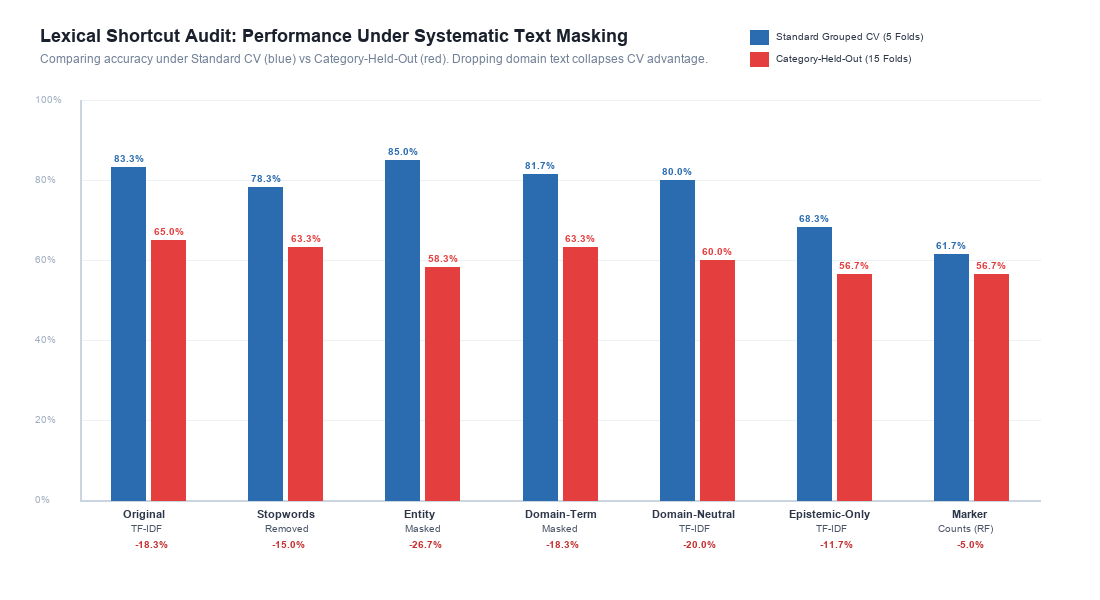
\includegraphics[width=\columnwidth]{figures/lexical_audit.png}
\caption{Performance across 7 systematic lexical masking transformations under Standard CV and Category-Held-Out protocols. Isolating epistemic tokens (ExpE) causes a $15.0\%$ drop in CV accuracy.}
\label{fig:lexical_audit}
\end{figure}

\begin{table*}[t]
\caption{Lexical Shortcut Audit Across 7 Text Transformations (TF-IDF Classifier)}
\label{tab:lexical_audit}
\centering
\begin{tabularx}{\textwidth}{llccccc}
\toprule
\textbf{Exp ID} & \textbf{Representation Condition} & \textbf{Standard CV Acc} & \textbf{Standard CV F1} & \textbf{Held-Out Acc} & \textbf{Held-Out F1} & \textbf{CV $\to$ Held-Out Drop} \\
\midrule
\textbf{ExpA} & \textbf{Original Full Text (Reference)} & $\mathbf{83.33\%}$ & $\mathbf{0.8365}$ & $\mathbf{65.00\%}$ & $\mathbf{0.6490}$ & $\mathbf{-18.33\%}$ \\
ExpB & Stopwords Removed (Epistemic Kept) & $78.33\%$ & $0.7836$ & $63.33\%$ & $0.6120$ & $-15.00\%$ \\
ExpC & Entity-Masked (Persons, Dates, Locations) & $85.00\%$ & $0.8525$ & $58.33\%$ & $0.5848$ & $\mathbf{-26.67\%}$ \\
ExpD & Domain-Term Masked (Jargon Stripped) & $81.67\%$ & $0.8189$ & $63.33\%$ & $0.6361$ & $-18.33\%$ \\
ExpG & Domain-Neutral (Entities \& Jargon Removed) & $80.00\%$ & $0.8030$ & $60.00\%$ & $0.5928$ & $-20.00\%$ \\
\textbf{ExpE} & \textbf{Epistemic-Only (Hedges, Modals, Refusals)} & $\mathbf{68.33\%}$ & $\mathbf{0.6606}$ & $\mathbf{56.67\%}$ & $\mathbf{0.5334}$ & $\mathbf{-11.66\%}$ \\
ExpF & Marker-Count Random Forest & $61.67\%$ & $0.6173$ & $56.67\%$ & $0.5656$ & $\mathbf{-5.00\%}$ \\
\bottomrule
\end{tabularx}
\end{table*}

As reported in Table~\ref{tab:generalization} and Fig.~\ref{fig:generalization_results}, when tested on held-out categories, TF-IDF + Linear SVM accuracy collapses from $83.33\%$ to $65.00\%$ ($-18.33\%$, exact binomial $p=0.000977$, 11 wins vs. 0 losses). Continuous sentence embeddings collapse even more severely (from $73.33\%$ to $48.33\%$), as latent embeddings cluster primarily by topical subject matter rather than epistemic mode.

Table~\ref{tab:lexical_audit} and Fig.~\ref{fig:lexical_audit} document the lexical masking experiments. Crucially, in \textbf{ExpE}, restricting the vocabulary strictly to epistemic markers (hedges, modals, refusals) causes standard CV accuracy to drop from $83.33\%$ to $68.33\%$ ($-15.00\%$, $p=0.0490$). This establishes that at least $15\%$ of the apparent performance of the single-response TF-IDF model is driven by non-epistemic domain content words (e.g., *mercury, treaty, kelvin*) correlated with ground truth labels rather than genuine uncertainty expressions.

\section{Discussion}

Our experimental investigation yields several key insights into the mechanics of LLM uncertainty estimation:

\subsection{Why Consistency Features Fail in Isolation}
A central finding is that \textsc{Consistency Only} features achieve only $50.0\%$ Accuracy and $0.460$ Macro-F1. Detailed error analysis indicates that cosine clustering on sentence embeddings struggles to decouple polysemic ambiguity from epistemic refusals. When an LLM encounters an unanswerable query (e.g., an unrecorded historical fact), stochastic sampling frequently produces diverse phrasing of refusal statements (e.g., ``Historical records do not preserve this datum'', ``It is unknown to modern scholarship''). Because the lexical structure varies, embedding-based clustering often segments these paraphrased refusals into multiple distinct clusters, artificially inflating semantic entropy and misclassifying \textsc{Unknown} queries as \textsc{Ambiguous}.

\subsection{The Variance Reduction Benefit of Multi-Sampling}
While semantic entropy alone is insufficient, multi-response sampling provides substantial empirical value ($+18.0\%$ Macro-F1 lift over single responses). However, our ablation study demonstrates that this benefit arises almost entirely from ensemble linguistic variance reduction. In a single response ($r_0$), an LLM may omit hedging due to decoding greed; across 10 samples, however, epistemic hesitation manifests consistently in length dispersion ($\sigma_{\text{len}}$) and cumulative negation counts. Aggregating linguistic features across samples provides a stable estimator that single responses cannot match.

\subsection{The Hazard of In-Domain Lexical Shortcuts}
Our findings issue a strong methodological caution regarding single-response uncertainty benchmarks. Bag-of-words models can achieve artificially high in-domain cross-validation accuracy ($83.33\%$) by memorizing topic-label correlations across balanced splits. Under rigorous Leave-One-Category-Out testing, these models collapse to $65.0\%$, and entity-masked models collapse to $58.3\%$. Multi-response sampling remains the only evaluated paradigm that does not rely on vocabulary memorization.

\section{Limitations}

We acknowledge several limitations in our study:
\begin{enumerate}
    \item \textbf{Dataset Scale:} Although Batch 2 Combined is rigorously balanced and annotated across 15 fine-grained categories ($N=60, M=600$), larger datasets ($N \ge 1,000$) will be necessary to train deep non-linear multi-task classifiers.
    \item \textbf{Single Generator Architecture:} Response generation was conducted using \texttt{Qwen3:4B}. While this isolated model-specific consistency properties, cross-model transferability across diverse model families (e.g., Llama, Mistral) requires further study.
    \item \textbf{Fixed Sampling Budget:} All multi-response experiments utilized a fixed budget of $M=10$ samples. Adaptive routing algorithms that allocate samples dynamically based on initial uncertainty warrant exploration.
\end{enumerate}

\section{Conclusion and Future Work}

We presented an empirical study of tri-class LLM uncertainty classification (\textsc{Known}, \textsc{Ambiguous}, \textsc{Unknown}) using multi-response consistency and linguistic features. Our results demonstrate that multi-response feature modeling achieves $80.0\%$ accuracy ($0.789$ Macro-F1), providing a statistically validated $+18.0\%$ lift over single-response baselines. However, feature ablations prove that consistency features do not outperform pure ensemble linguistic aggregation, indicating that variance reduction over lexical markers drives the multi-response performance advantage. Finally, Leave-One-Category-Out audits reveal that single-response bag-of-words models suffer severe domain generalization collapse, emphasizing the critical importance of category-held-out protocols when evaluating uncertainty quantification in natural language processing. Future work will investigate dynamic sampling allocations and cross-model calibration.

\bibliographystyle{IEEEtran}
\bibliography{references}

\end{document}
